\documentclass[convert = false, tikz]{standalone}
\usepackage[utf8]{inputenc}
\usepackage{tikz}
\usetikzlibrary{automata, positioning, arrows}
 
\usepackage{../../../../style_automata}

\begin{document}
    \tikzset{
    node distance=2.5cm, % specifies the minimum distance between two nodes.
    }
    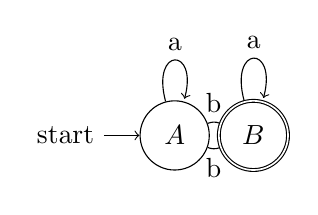
\begin{tikzpicture}
        \node[state, initial] (a) {$A$};
        \node[state, accepting, right of=a] (b) {$B$};
        \draw (a) edge[loop above] node{a} (a)
        (a) edge[above, bend left=20] node{b} (b)
        (b) edge[loop above] node{a} (b)
        (b) edge[below, bend left=20] node{b} (a)
        ;
    \end{tikzpicture}
\end{document}
